\documentclass[a4paper, 12pt]{article}

\usepackage{amsfonts} % if you want blackboard bold symbols e.g. for real numbers
\usepackage{graphicx} % if you want to include jpeg or pdf pictures
\usepackage{wrapfig}
\usepackage{caption}
\usepackage{subcaption}
\usepackage{float}
\usepackage{hyperref}
\usepackage{amsmath}

\title{Project 1 - Image Segmentation} % change this
\author{Ankit Arya} % change this
\date{\today} % change this

\begin{document}

%%%%%%%%%% PRELIMINARY MATERIAL %%%%%%%%%%
\maketitle
\begin{center}
ECE-8493 - Introduction to Neural Networks. % change this
\\[12pt]
Taught by Dr.\ Jenny Du. % change this
\end{center}
\thispagestyle{empty}


%%%%%%%%%% MAIN TEXT STARTS HERE %%%%%%%%%%

%%%%%%%%%% SAMPLE SECTION %%%%%%%%%%
\newpage
\section{Technical Description}
%

Note-  This description is put together using \url{"http://ufldl.stanford.edu/wiki/index.php/Neural_Networks"} as a major resource. The equations present in the resource also guide my implementation of neural networks.
\\~\\

A neural network is constructed by connecting neurons to one another, such that output of a neuron can be the input of another. For example, here is a small neural network:

\begin{figure}[H]
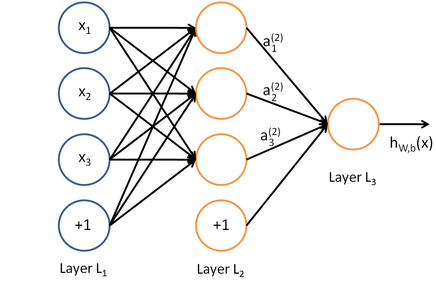
\includegraphics[scale=0.5]{nNetwork}
\caption{Neural Network with 3 input units, 3 hidden units, and one output.}
\end{figure}


\subsection{Forward Propogation}
$x_1,x_2,x_3.....$ are the inputs. 
Weights are defined as$W$, where $W^l_{ij} $ denotes the parameter (or weight) associated with the connection between unit j in layer l, and unit i in layer l + 1. We will write $a^{(l)}_i $ to denote the activation (meaning output value) of unit i in layer l. For l = 1, we also use $a^{(l)}_i = x_i$   to denote the $i-th$ input. Given a fixed setting of the parameters W,b, neural network defines a hypothesis $h_{W,b}(x)$ that outputs a real number.
 Also lets $z^{(l)}_i $  denote the total weighted sum of inputs to unit i in layer l, including the bias term. $f(.)$ is the sigmoid activation function.
Equations of $forward$ $propogation$ can be represented compactly as:

\begin{alignat}{2}
z^{(l+1)}= W^{(l)} x+ b^{(1)} \\
a^{(l+1)}= f(z^{(l+1)})
\end{alignat} 


\subsection{Backpropopogation Algorithm}
%
Given a training set of m examples, the overall cost function can be defined as:

\begin{figure}[H]
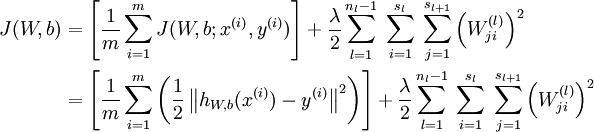
\includegraphics[scale= 0.5]{eq}
\end{figure}

The goal is to minimize the above stated cost function using batch gradient descent or other advanced optimization algorithm.

The weight decay parameter $\lambda$ controls the relative importance of the two terms. Note also the slightly overloaded notation: $J(W,b;x,y)$ is the squared error cost with respect to a single example; $J(W,b)$ is the overall cost function, which includes the weight decay term.


Step by step process algorithm is shown below:

\begin{enumerate}
\item Perform a feedforward pass, computing the activations for layers , , up to the output layer , using the equations defining the forward propagation steps.

\item For the output layer (layer $n_l$ ), set

   $ \delta^{n_l}= - (y - a^{(n_l)}).*f'(z^{(l)})$
\item For $l =n_l -1. n_l -2, ...$

Set

$\delta^l = ((W^{l})^T\delta^{(l+1)}).*f'(z^{(l)})$

\item Compute the desired partial derivates:
	
$\nabla_{W^l}J(W,b;x,y) =\delta^{(l+1)}(a^l)^T,$

$\nabla_{b^l}J(W,b;x,y) =\delta^{(l+1)}$
	
\end{enumerate}

\newpage
%%%%%%%%%% INFORMATION %%%%%%%%%%
\section{ Neural net Implementation }

Project is executed by running the file $main.m$

Steps  to train the network:

\begin{enumerate}
 
  \item Specify parameters used:

input\_layer\_size =3    ( total of 900 training samples)

hiddlen\_layer\_size =3

num\_labels= 3   ( 3 assigned classes: flowers, leaves, background)

  \item Randomly intialize Weights to train the network - $ Theata1 and Theta2$
  \item Set value for max\_iteration and the regularization parameter $lambda$.
		Value used: 
			
				$max\_iter=300$
	
				$lambda=1$

neural net stops when number of iterations are completed.
 \item Training the network includes call to the nnCostFunction using sigmoid activation, which includes implementation of the feed forward and the backpropogation algorithm . The functions returns the optimized value of the weights which are used for prediciton.

\item Once Theta1 and Theta2 are returned,   function in predict.m is called.

$[p, soft\_class] = PREDICT(Theta1, Theta2, testData)$ outputs the predicted label of testData given the
   trained weights of a neural network $(Theta1, Theta2)$

p is the hard classification result, where as soft\_class contains the soft classification map.
 \end{enumerate}

NOTE - Learning rate is not chosen manually, as instead of implementing Gradient Descent I have used an advanced optimizer $fmincg$. These
 advanced optimizers are able to train our cost/loss functions efficiently as long as we provide them with the gradient computations.


\newpage

\section{Results}

Image Segmentations results are shown as follows:

\begin{figure}[H]
  \centering
  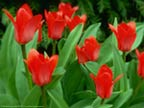
\includegraphics[width=4in]{flowers}
  \caption{Orignal Image}
\end{figure}
 


\begin{figure}[H]
        \centering
        \begin{subfigure}[b]{0.3\textwidth}
                \centering
                
\includegraphics[width=\textwidth]{flower}
                \caption{Flowers}
                \label{fig:gull}
        \end{subfigure}%
        ~ %add desired spacing between images, e. g. ~, \quad, \qquad etc. 
          %(or a blank line to force the subfigure onto a new line)
        \begin{subfigure}[b]{0.3\textwidth}
                \centering
                
\includegraphics[width=\textwidth]{leaves}
                \caption{Leaves}
                \label{fig:tiger}
        \end{subfigure}
        ~ %add desired spacing between images, e. g. ~, \quad, \qquad etc. 
          %(or a blank line to force the subfigure onto a new line)
        \begin{subfigure}[b]{0.3\textwidth}
                \centering
                
\includegraphics[width=\textwidth]{bckgrnd}
                \caption{Background}
                \label{fig:mouse}
        \end{subfigure}
        \caption{Image Segmentation}\label{fig:animals}
\end{figure}

For hard classification and and soft classification maps please see the section below.

\section{Matlab Code}

Matlab code is attached as a tarball with email. Main.m is the file that is used to run the program. Resulting segmentations  are stored as flower, learves, and background ( all PNG files). Hard and soft classification maps are stored as hard\_map.mat and soft\_map.mat.

%%%%%%%%%% BIBLIOGRAPHY %%%%%%%%%%
\section*{Bibliography}
%



1. Ng, Andrew, and Jiquan Ngiam. "UFLDL Tutorial - Ufldl." Unsupervised Feature Learning and Deep Learning. N.p., n.d. Web. 25 Sept. 2012. \url{"http://ufldl.stanford.edu/wiki/index.php/UFLDL\_Tutorial"}


\end{document}
